\documentclass[border=3pt,varwidth]{standalone}
\usepackage{amsmath,amssymb}
\usepackage{tikz}
\usetikzlibrary{arrows.meta,calc,decorations.markings,patterns,positioning,angles,quotes}
\tikzset{
  >=Stealth,
  every node/.style={font=\normalsize},
  wire/.style={line width=0.9pt},
  thinwire/.style={line width=0.6pt},
  fieldline/.style={line width=0.6pt,-{Stealth[length=2.2mm]}},
  axis/.style={line width=0.7pt,-{Stealth[length=2.2mm]}},
  dashedwire/.style={line width=0.9pt,dash pattern=on 3pt off 2pt},
  resistor/.style={line width=0.9pt},
  chargepos/.style={circle,draw,line width=0.8pt,minimum size=5mm,inner sep=0pt},
  dotcharge/.style={circle,fill,inner sep=0pt,minimum size=2.4pt}
}
% Draw a resistor box centered at (x,y) with width w, height h, horizontal
\newcommand{\resbox}[4]{%
  % #1=x #2=y #3=halfwidth #4=label
  \draw[resistor] (#1-#3,#2-0.18) rectangle (#1+#3,#2+0.18);
  \ifx\\#4\\\else\node[above=2pt] at (#1,#2+0.18) {#4};\fi
}
% Battery symbol: long thin line (+) then short thick line (-), centered at (x,y)
\newcommand{\battery}[2]{%
  % #1=x #2=y ; long line left=+, short line right=- by default orientation
  \draw[wire] (#1-0.09,#2-0.32) -- (#1-0.09,#2+0.32);
  \draw[line width=2.6pt] (#1+0.09,#2-0.16) -- (#1+0.09,#2+0.16);
}

\begin{document}
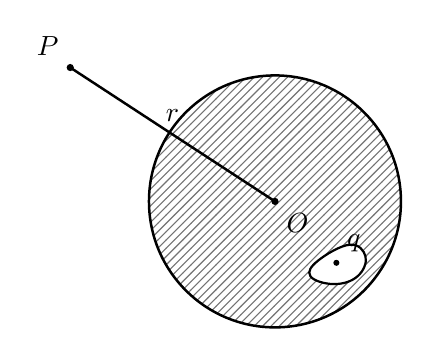
\begin{tikzpicture}[scale=1]
  \def\R{1.6}
  \filldraw[pattern=north east lines, pattern color=black!55, draw=black, line width=0.9pt] (0,0) circle (\R);
  % irregular cavity near lower-right, drawn as a smooth blob
  \filldraw[fill=white, draw=black, line width=0.8pt]
    plot [smooth cycle, tension=0.7] coordinates {
      (0.55,-0.75) (0.95,-0.55) (1.15,-0.70) (1.05,-0.95)
      (0.75,-1.05) (0.45,-0.95)
    };
  \node (q) at (0.78,-0.78) {};
  \fill (q) circle (1.1pt);
  \node[above right=0.5pt] at (q) {$q$};
  \fill (0,0) circle (1.3pt);
  \node[below right=1pt] at (0,0) {$O$};
  \coordinate (P) at (-2.6,1.7);
  \fill (P) circle (1.3pt);
  \node[above left=1pt] at (P) {$P$};
  \draw[wire] (P) -- (0,0);
  \node[above=1pt] at ($(P)!0.5!(0,0)$) {$r$};
\end{tikzpicture}
\end{document}
